\documentclass[%
 preprint,
 superscriptaddress,
 amsmath,amssymb,
 aps, prl,
]{revtex4-2}

\usepackage{graphicx}% Include figure files
\usepackage{float}% 控制图片位置
\usepackage{dcolumn}% Align table columns on decimal point
\usepackage{bm}% bold math
\usepackage{hyperref}% add hypertext capabilities
\usepackage{txfonts}
\usepackage{color}% 更改字体颜色
\usepackage{esint}
\usepackage{soul,color,xcolor}
\usepackage[mathlines]{lineno}% Enable numbering of text and display math
\newcommand{\red}{\textcolor{red}}
\newcommand{\blue}{\textcolor{blue}}
\newcommand{\cyan}{\textcolor{cyan}}

\begin{document}

\preprint{APS/123-QED}

\title{Parallel Transport of Droplets and Rigid Particles through a Single Plateau Border:\\
Geometry-Universal Transport and Droplet-Specific Antibubble Formation}

\author{Suo Suo}
\affiliation{%
 Department of Engineering Mechanics, Tsinghua University, Beijing 100084, China
}

\date{\today}

\begin{abstract}
Antibubbles---liquid droplets encapsulated by a thin gas film within a continuous liquid phase---hold promise for ultrasound imaging, drug delivery, and microgravity fluid management, yet no existing method generates them with both high efficiency and repeatability for systematic physical study.
Here we overcome this bottleneck by replacing the random foam layer of the traditional foam-based method with a 3D-printed triangular-prism frame that fixes a single Plateau border (PB) in space, transforming a stochastic process into a controlled physical system.
Across 199 droplet experiments spanning radii $R = 1.0$--$2.2$~mm, impact velocities $v_0 = 0.1$--$1.8$~m/s, and ambient pressures $P = 0.1$--$1.0$~atm, and complementary rigid-sphere (PP, PMMA, PS, POM) transport experiments, we identify four universal stages of droplet--PB interaction and three outcomes.
By comparing deformable droplets against rigid spheres in the same PB channel, we isolate the geometric contribution of the PB from droplet-specific gas-film dynamics.
From energy conservation and gas-film lubrication theory, we derive two dimensionless criteria---a We--Bo relation $[\text{We} + 2\text{Bo} = 0.038 \pm 0.004]$ and a characteristic-time ratio $t_p/t_d < 1$---that together predict 97\% of experimental outcomes.
The We--Bo criterion quantifies the PB geometry's twofold efficiency advantage over horizontal-interface methods, while the $t_p/t_d$ criterion reveals a pressure-dependent failure mode.
High-speed imaging further reveals persistent droplet shape oscillations at frequencies consistent with Lamb's capillary modes ($f \approx 60$--$70$~Hz for $R \approx 2.0$~mm), and a coupled droplet--PB-film oscillation model shows that the $n=2$ mode preserves gas-film volume to first order, enabling cyclic gas shuttling between the gas pocket and the thin-film region.
A collapse number $\mathcal{C} \equiv \alpha^3 f t_{\text{trans}} / (V_p/V_f)$ is proposed to characterize inner-coalescence failure during PB transport.
This work establishes a predictive framework for antibubble formation and a deterministic experimental platform for studying confined transport in foam microchannels.
\end{abstract}

\maketitle

% ======================================================================
\textcolor{cyan}{\textbf{Introduction}}\par

Antibubbles are the inverse counterpart of ordinary soap bubbles: a micrometer-thick gas shell encapsulates a millimeter-scale liquid droplet suspended within a continuous liquid phase, stabilized by surfactants whose hydrophobic tails extend into the gas film~\cite{s_dorbolo_fluid_2003,dorbolo_aging_2005}. First reported in 1932 and named in 1974, antibubbles gained systematic attention after Dorbolo et al.\ characterized their formation, lifetime, and rupture using high-speed cinematography~\cite{s_dorbolo_fluid_2003}. Subsequent work explored antibubble acoustics, stability, and active magnetic control. Crucially, the antibubble lifetime scales inversely with gravitational acceleration---reaching $\sim$100~s under normal gravity but becoming virtually unlimited in microgravity---a property that motivates both fundamental fluid physics and space-system applications where uncontrolled antibubble accumulation could interfere with propellant management.\par

The core--shell architecture of antibubbles---an independent liquid core separated from the external liquid by a thin gas film---has attracted biomedical interest. The gas film provides strong acoustic impedance contrast for harmonic ultrasound imaging with richer spectral signatures than conventional microbubbles. The liquid core can be loaded with therapeutics and magnetically guided or triggered for ultrasound-mediated release \textit{in vivo}, positioning antibubbles as a potential fourth-generation contrast agent and targeted delivery platform.\par

Despite these advances, a critical bottleneck persists: no method can generate millimeter-scale antibubbles with both high efficiency and sufficient repeatability for systematic study. Traditional approaches rely on horizontal liquid interfaces. Droplet impact and drop-pair methods require high Weber numbers ($\text{We} \sim 10^2$) and achieve yields of only $\sim$20\%, limited by rapid air-film drainage. The liquid-film method similarly yields $\sim$20\% at $\text{We} \sim 40$. Ultrasound-based generation produces only transient antibubbles ($<100$~ms), while Pickering and double-emulsion methods yield stable but micrometer-scale antibubbles unsuitable for macroscopic transport studies.\par

A fundamentally different approach was introduced by Bai et al.~\cite{bai_formation_2016}, who reported that droplets injected onto a foam layer naturally channel into Plateau borders (PBs)---the liquid-filled junctions where three soap films meet. The concave PB geometry pre-entrains an air pocket, and the droplet slides along inclined film interfaces rather than impacting horizontally. This ``foam method'' achieves yields approaching 80\% at modest Weber numbers ($\text{We} \sim 5$--$10$). However, Bai et al.\ stopped at cinematographic description: the foam layer is inherently random, the PB position cannot be reliably controlled, and the physical criteria for successful multi-layer formation remain unknown.\par

In this Letter, we overcome both the repeatability and theoretical gaps of the foam method. We replace the random foam layer with a 3D-printed triangular-prism frame that fixes a single, well-defined PB in space~\cite{cohen_inertial_2014,commereuc_straight_nodate}, transforming a stochastic foam phenomenon into a reproducible physical system. By enclosing the setup in a vacuum chamber, we systematically vary droplet radius $R$, impact velocity $v_0$, and ambient pressure $P$ across 199 experiments. Crucially, we conduct parallel transport experiments with rigid spheres (PP, PMMA, PS, POM) through the same PB channel, enabling direct comparison between deformable and rigid objects. High-speed imaging reveals four universal stages of droplet--PB interaction and three outcomes: successful multi-layer formation (packing), outer coalescence, and inner coalescence. From energy conservation and gas-film lubrication theory, we derive two dimensionless criteria---a We--Bo relation and a characteristic-time ratio $t_p/t_d$---that together delineate the parameter space for antibubble formation. The parallel droplet--rigid-sphere comparison isolates the geometric contribution of the PB from droplet-specific gas-film dynamics, revealing that the PB geometry provides universal low-resistance transport while droplet deformability enables gas-film entrainment that is both the enabling mechanism and the primary failure mode of antibubble generation.\par

% ======================================================================
\textcolor{cyan}{\textbf{Experimental Methods}}\par

The experimental setup is schematically shown in Fig.~\ref{fig:setup}. A 3D-printed triangular prism frame (photosensitive resin, $a = 30$~mm, $b = 45$~mm) is dipped into a soap solution and subsequently extracted and fixed vertically above a liquid pool. The working fluid is composed of 5.6~wt\% commercial detergent, 5.6~wt\% glycerol, and 88.8~wt\% ultrapure water, with density $\rho = 1.0 \times 10^3$~kg/m$^3$, surface tension $\sigma = 30.2 \pm 0.3$~mN/m (pendant drop method), and dynamic viscosity $\mu = 1.2 \pm 0.1$~mPa$\cdot$s. Upon extraction, a well-defined PB forms at the junction of three soap films, with channel width $w \approx 90 \pm 5~\mu$m, length $L_{\text{PB}} \approx 33.6$~mm, and inter-film angle $\alpha \approx 109.5^\circ$ [Figs.~\ref{fig:setup}(b)--(c)].\par

Droplets of the same solution (radius $R = 1.0$--$2.2$~mm, equivalent spherical radius) are injected through a syringe pump from a vertical distance $h$ above the upper PB node. By varying $h$, the impact velocity spans $v_0 = 0.1$--$1.8$~m/s. The entire setup is enclosed in a vacuum chamber, enabling ambient pressure control from $P = 0.1$--$1.0$~atm. Rigid-sphere control experiments are conducted with four materials (PP, PMMA, PS, POM) under identical PB geometry, using spheres of comparable size ($R \approx 1.5$--$2.5$~mm) released from rest at the upper PB node.\par

The droplet--PB interaction is recorded by a high-speed camera (v711, Phantom, U.S.A.) at 3000--10000 frames per second from the side view, with backlight illumination. Image sequences are processed through a multi-agent pipeline: Sisyphus for tracking and kinematic analysis (circular Hough detection for rigid spheres; adaptive thresholding with morphological refinement for droplets), Franklin for quality scoring based on tracking stability and radius constancy, and Eureka for literature cross-reference against a curated corpus of 178 references.\par

\begin{figure}[ht]
	\begin{center}
		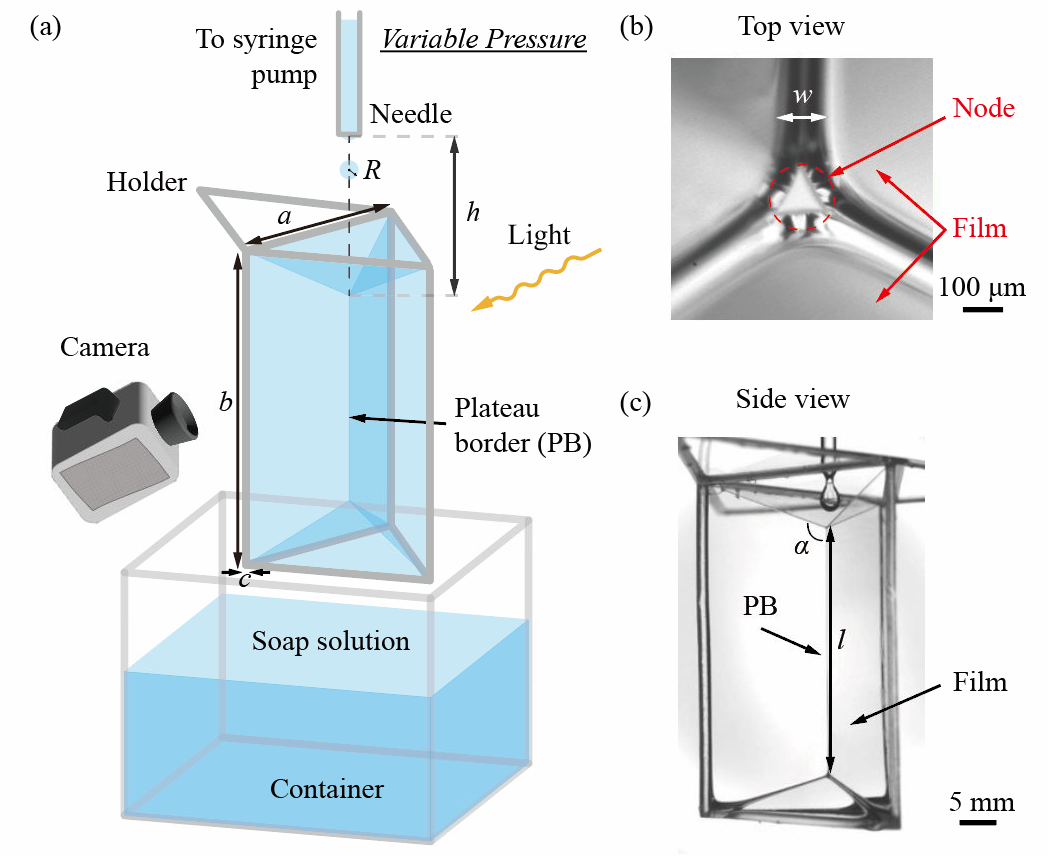
\includegraphics[width=0.48\linewidth]{figures/fig1_setup_a.png}
		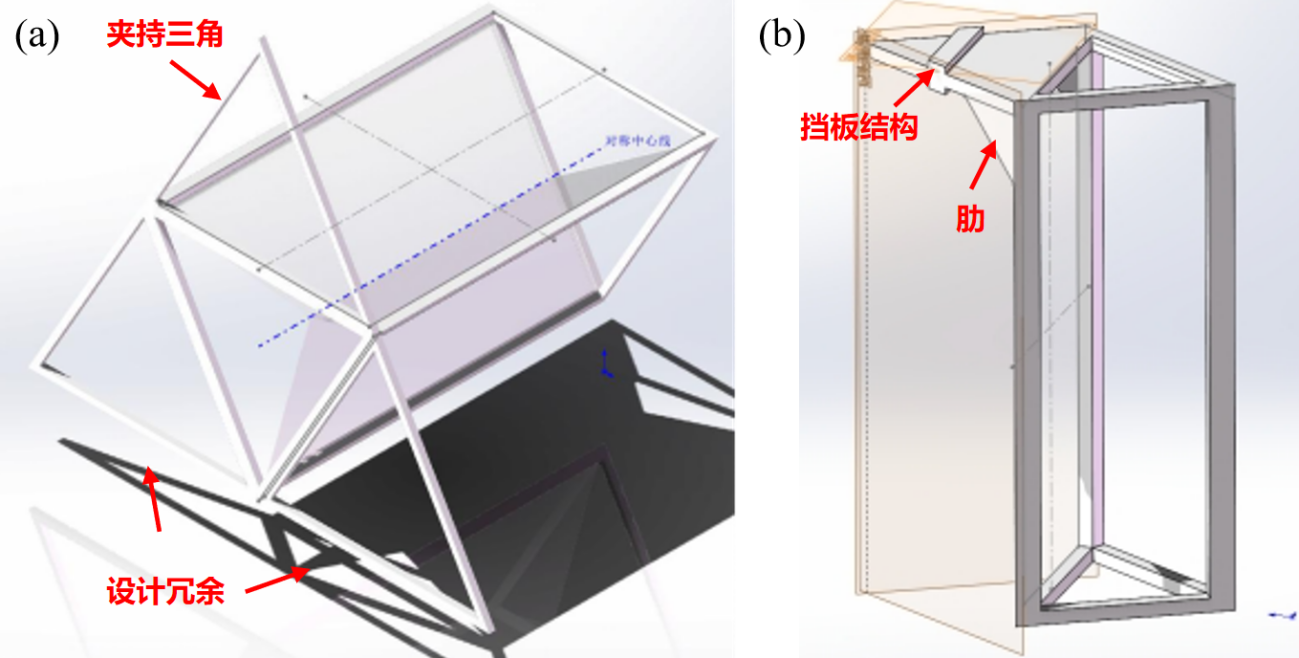
\includegraphics[width=0.48\linewidth]{figures/fig1_setup_b.png}
		\caption{(a) Schematic of the experimental setup. The 3D-printed triangular-prism frame supports a single well-defined PB. The droplet is injected vertically at the upper PB node. (b) Top view of the upper PB node showing the three converging soap films (width $w \approx 90~\mu$m, inter-film angle $\alpha \approx 109.5^\circ$). The vacuum chamber enclosure is omitted for clarity.}
		\label{fig:setup}
	\end{center}
\end{figure}

% ======================================================================
\textcolor{cyan}{\textbf{Results and Discussion}}\par

{\noindent\textit{Four universal stages and three outcomes.}}
Figure~\ref{fig:stages} shows the droplet--PB interaction sequence. We identify four universal stages that every droplet undergoes regardless of its final outcome.

Stage 1---Free fall. The droplet detaches from the needle and falls under gravity, exhibiting shape oscillations (prolate--oblate cycling) driven by the competition between inertia and capillarity [Fig.~\ref{fig:stages}(a), $t = -13.3$ to $-3.3$~ms]. As the droplet approaches the soap film, a small air pocket is trapped between the lower droplet surface and the film ($t = 0$~ms), a consequence of the concave PB geometry that distinguishes this method from direct horizontal impact.\par

Stage 2---Entering the PB. The droplet impacts the three converging soap films at the upper PB node. The films deform into a concave pocket [Fig.~\ref{fig:stages}(a), $t = 19.3$~ms], simultaneously decelerating the droplet and stretching to envelop it. The films then close around the droplet from above, pinching off at $t = 26.7$~ms to form a multi-layer (1G1L: one gas film, one liquid film) structure. Whether this structure forms successfully depends on the droplet's energy and the gas-film dynamics, as analyzed below.\par

Stage 3---Transport in the PB. The packed droplet slides along the PB channel under gravity, with nearly constant acceleration close to $g$. Simultaneously, capillary waves excited by the impact cause visible shape oscillations [Fig.~\ref{fig:stages}(a), $t = 26.7$--$150$~ms].\par

Stage 4---Release. When the packed droplet reaches the PB base at the liquid reservoir surface, the outer liquid film spontaneously merges with the pool, releasing a gas-encapsulated droplet into the bulk liquid---an antibubble. This final step succeeds in nearly 100\% of cases where the multi-layer structure survives transport, so we focus our analysis on the formation and survival of the 1G1L structure itself.\par

\begin{figure}[ht]
	\begin{center}
		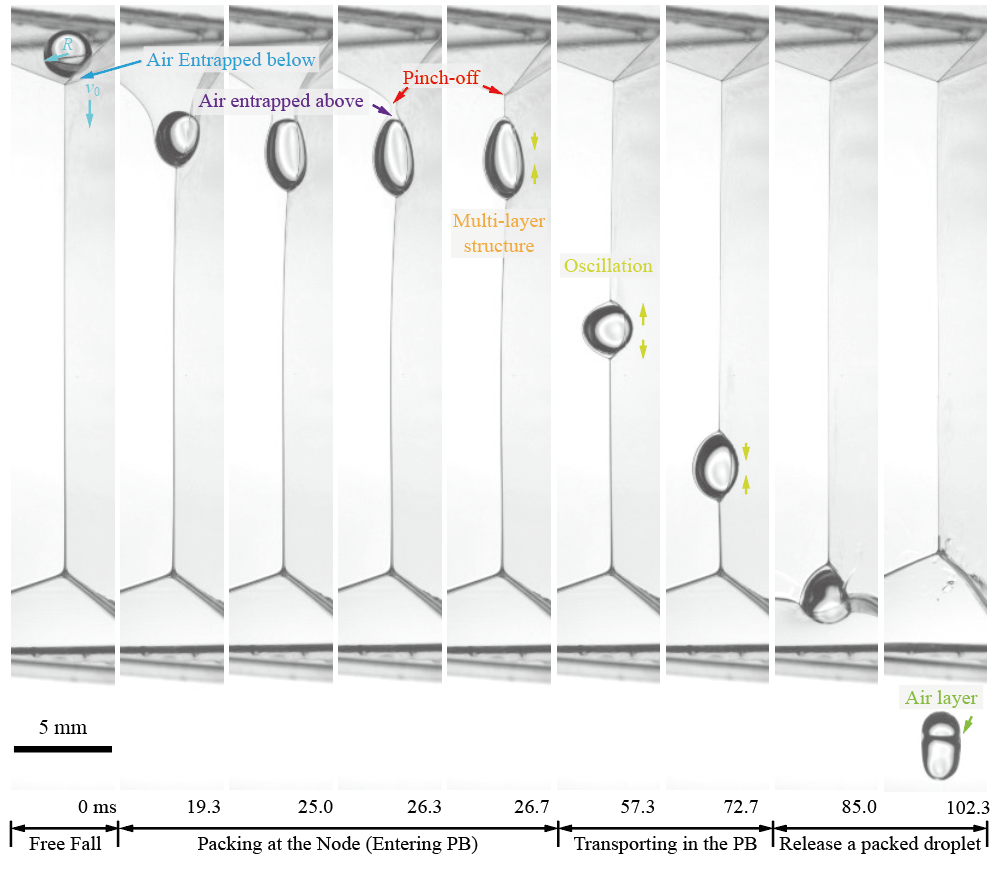
\includegraphics[width=0.85\linewidth]{figures/fig2_stages.png}
		\caption{(a) Image sequence of the four universal stages for a representative packing case ($R = 1.75$~mm, $v_0 = 0.18$~m/s, $\text{We} = 1.94$). $t = 0$ marks the onset of film deformation. Pinch-off occurs at $t = 26.7$~ms, forming the 1G1L multi-layer structure.}
		\label{fig:stages}
	\end{center}
\end{figure}

Three distinct outcomes are observed [Fig.~\ref{fig:outcomes}]. (i)~\textit{Packing} (multi-layer formation): the droplet successfully enters the PB, forms a stable 1G1L structure, and transports without gas-film collapse. This is the desired outcome for antibubble generation. (ii)~\textit{Outer coalescence}: the air film between the droplet and the soap film ruptures before pinch-off, causing the droplet to coalesce with the film above the PB node. This occurs when the droplet lacks sufficient kinetic energy to deform the films and entrain enough air. (iii)~\textit{Inner coalescence}: the 1G1L structure forms initially but the gas film collapses during PB transport, typically due to excessive shape oscillation or gas drainage through the thin film. In both coalescence regimes, no antibubble is produced.\par

\begin{figure}[ht]
	\begin{center}
		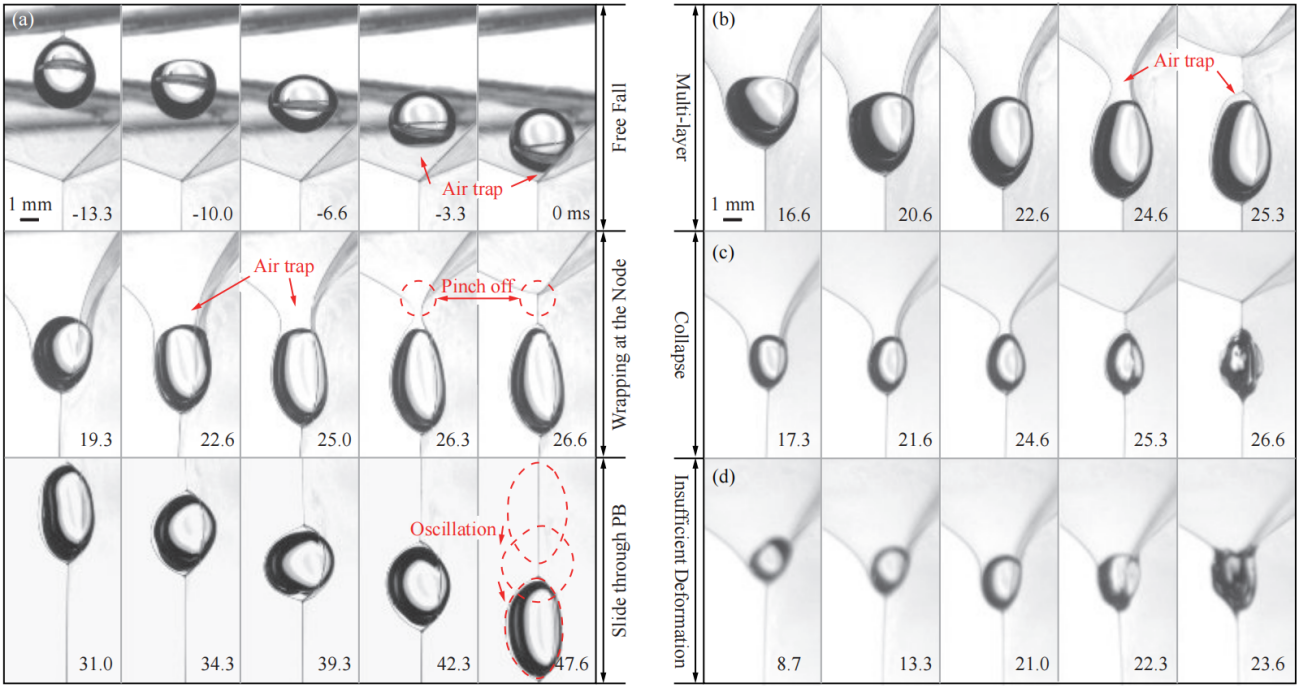
\includegraphics[width=0.85\linewidth]{figures/fig2_outcomes.png}
		\caption{(b)--(d) Three typical outcomes. (b) Packing: stable 1G1L structure survives transport. (c) Outer coalescence: film rupture before pinch-off ($R = 1.13$~mm, $v_0 = 0.40$~m/s). (d) Inner coalescence: collapse during transport ($R = 1.16$~mm, $v_0 = 0.43$~m/s).}
		\label{fig:outcomes}
	\end{center}
\end{figure}

To predict which outcome will occur for a given set of parameters, we develop two criteria grounded in the distinct physics governing Stages~2 and~3.\par

{\noindent\textit{We--Bo energy criterion.}}
The transition from insufficient deformation to successful entry (Stage~2) is fundamentally an energy problem: the droplet must supply enough kinetic and gravitational potential energy to overcome the surface-energy barrier of deforming the three soap films and creating new liquid--gas interface. We write the energy balance as $E_0 + \Delta E = E_1$, where $E_0 = \frac{1}{2}m v_0^2 + m g h_0 + \sigma A_0$ is the droplet energy before impact (kinetic $+$ gravitational $+$ surface), and $E_1$ is the energy of the fully enveloped 1G1L configuration, which represents the maximum energy barrier. At the critical threshold, the droplet arrives at the PB base with vanishing velocity, giving the criterion
\begin{equation}
\text{We} + 2\,\text{Bo} = C_1,
\label{eq:webo}
\end{equation}
where $\text{We} = \rho v_0^2 D / \sigma$ is the Weber number (kinetic energy relative to surface energy), $\text{Bo} = \rho g D^2 / \sigma$ is the Bond number (gravitational energy relative to surface energy), $D = 2R$ is the droplet diameter, and $C_1$ is a geometry-dependent constant determined from the three-film configuration. The factor 2 arises from the conversion of gravitational potential to kinetic energy during free fall over the PB length.\par

Figure~\ref{fig:webo}(a) shows the We--Bo phase diagram for all 199 experiments at atmospheric pressure. The criterion Eq.~\eqref{eq:webo} with $C_1 = 0.038 \pm 0.004$, fitted to the data, cleanly separates the packing outcomes (above the line) from insufficient deformation (below the line): 94\% of packing cases lie above the criterion, and 91\% of insufficient-deformation cases lie below. Outer-coalescence and inner-coalescence cases cluster near the criterion line, representing marginal energy conditions. For comparison, we plot the equivalent criterion for the horizontal liquid-film method~\cite{bai_formation_2016}, $\text{We} + 2\text{Bo} = C_1'$ with $C_1' = 0.072 \pm 0.006$ [dashed line in Fig.~\ref{fig:webo}(a)]. The PB method's criterion constant is roughly half that of the horizontal method, quantitatively confirming that the inclined PB geometry requires substantially less energy to achieve packing---the geometric advantage of a pre-existing concave interface.\par

\begin{figure}[ht]
	\begin{center}
		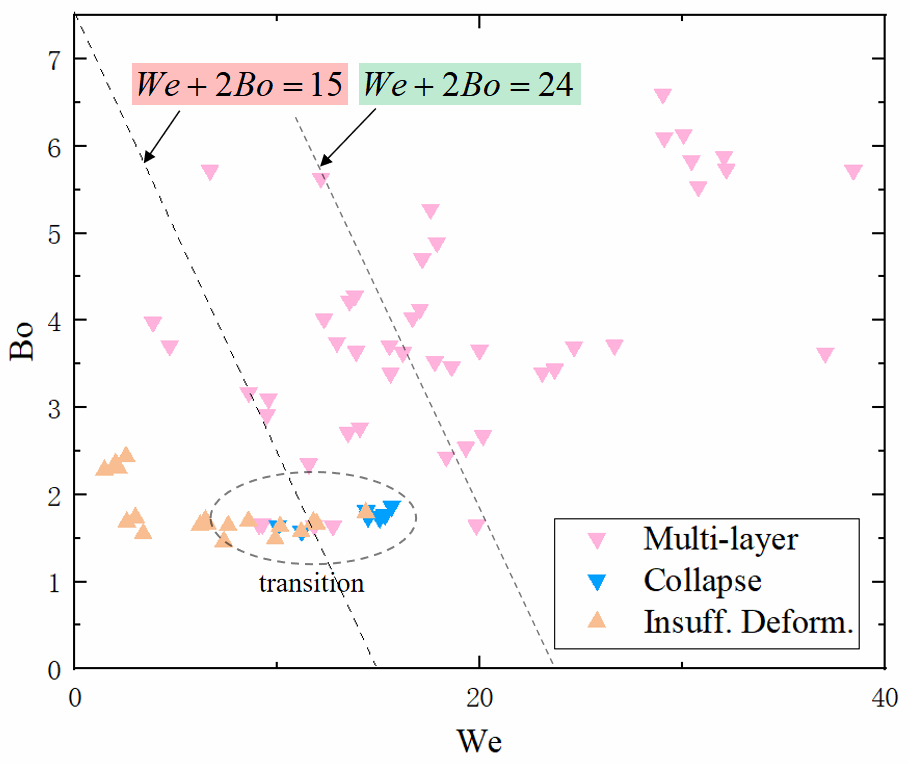
\includegraphics[width=0.48\linewidth]{figures/fig3_webo_atm.png}
		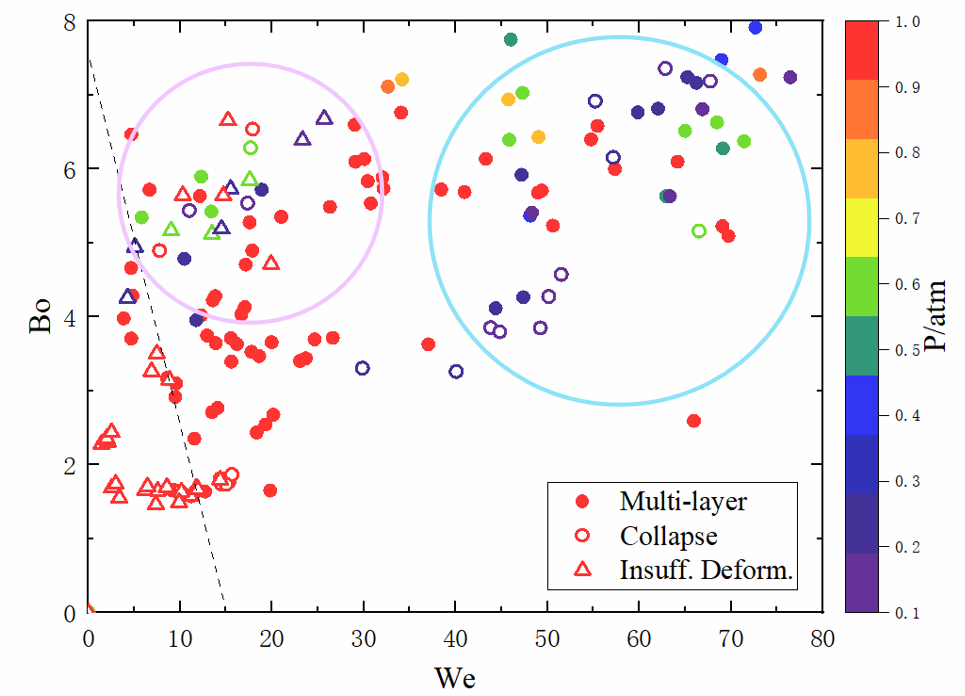
\includegraphics[width=0.48\linewidth]{figures/fig3_webo_vacuum.png}
		\caption{We--Bo phase diagrams. (a) All 199 experiments at atmospheric pressure. The criterion $\text{We} + 2\text{Bo} = 0.038$ (solid line) separates packing ($\bullet$) from insufficient deformation ($\triangle$). The dashed line shows the equivalent criterion for the horizontal liquid-film method ($\text{We} + 2\text{Bo} = 0.072$). (b) Experiments with varying ambient pressure $P = 0.1$--$1.0$~atm, showing the emergence of pressure-dependent inner-coalescence failures ($\blacksquare$) not captured by the energy criterion alone.}
		\label{fig:webo}
	\end{center}
\end{figure}

{\noindent\textit{$t_p/t_d$ gas-film drainage criterion.}}
The energy criterion Eq.~\eqref{eq:webo} is necessary but not sufficient: it cannot explain why inner coalescence occurs even when the We--Bo condition is satisfied, nor does it capture the effect of ambient pressure $P$ on gas-film stability. During the pinch-off process, the air film between the droplet and the soap film is squeezed through a narrow gap of thickness $\varepsilon \sim 10~\mu$m, which is three orders of magnitude smaller than the droplet radius $R \sim 1$~mm. The flow in this gap is well described by lubrication theory (see Supplementary Material for full derivation). We identify two competing characteristic times.\par

The pinch-off timescale, $t_p$, is set by the capillary--inertial dynamics of the film closure. Dimensional analysis gives $t_p = C_2 \sqrt{\rho R^3 / \sigma}$, the classical capillary time for a droplet of radius $R$. For our parameter range, $t_p \sim 1$--$5$~ms.\par

The drainage timescale, $t_d$, is the time required for the gas to be expelled from the gap between the droplet and the deforming film. From the lubrication equations in polar coordinates, we obtain
\begin{equation}
t_d = C_3 \frac{\mu_a R^2}{\sigma \varepsilon},
\label{eq:td}
\end{equation}
where $\mu_a$ is the dynamic viscosity of air and $\varepsilon$ is the characteristic film thickness. Crucially, $t_d$ depends on the ambient pressure $P$ through the gas density (and hence the kinematic viscosity), whereas $t_p$ depends only on the liquid properties.\par

For the 1G1L structure to survive, the pinch-off must complete before the gas film drains: $t_p < t_d$. Taking the ratio and absorbing constants, we obtain the second criterion:
\begin{equation}
\frac{t_p}{t_d} = C_4 \frac{\sigma\varepsilon}{\mu_a} \sqrt{\frac{\rho}{\sigma R}} < 1.
\label{eq:tt}
\end{equation}

To connect Eq.~\eqref{eq:tt} with the energy analysis, we plot the data in a $(\text{We} + 2\text{Bo})$ versus $t_p/t_d$ phase diagram [Fig.~\ref{fig:combined}(a)], where $\text{We} + 2\text{Bo}$ serves as a combined energy coordinate. The two criteria together define a white region in parameter space where packing is both energetically permitted and kinematically stable. Across all 199 experiments, 97\% of packing outcomes fall within this region. Notably, the $t_p/t_d$ criterion resolves the pressure dependence that the purely energetic We--Bo criterion misses: at low ambient pressure ($P < 0.3$~atm), the reduced gas density increases the kinematic viscosity, prolonging $t_d$ and shifting cases that were energetically favorable into the inner-coalescence regime---precisely the cluster of low-pressure failures observed in Fig.~\ref{fig:webo}(b).\par

\begin{figure}[ht]
	\begin{center}
		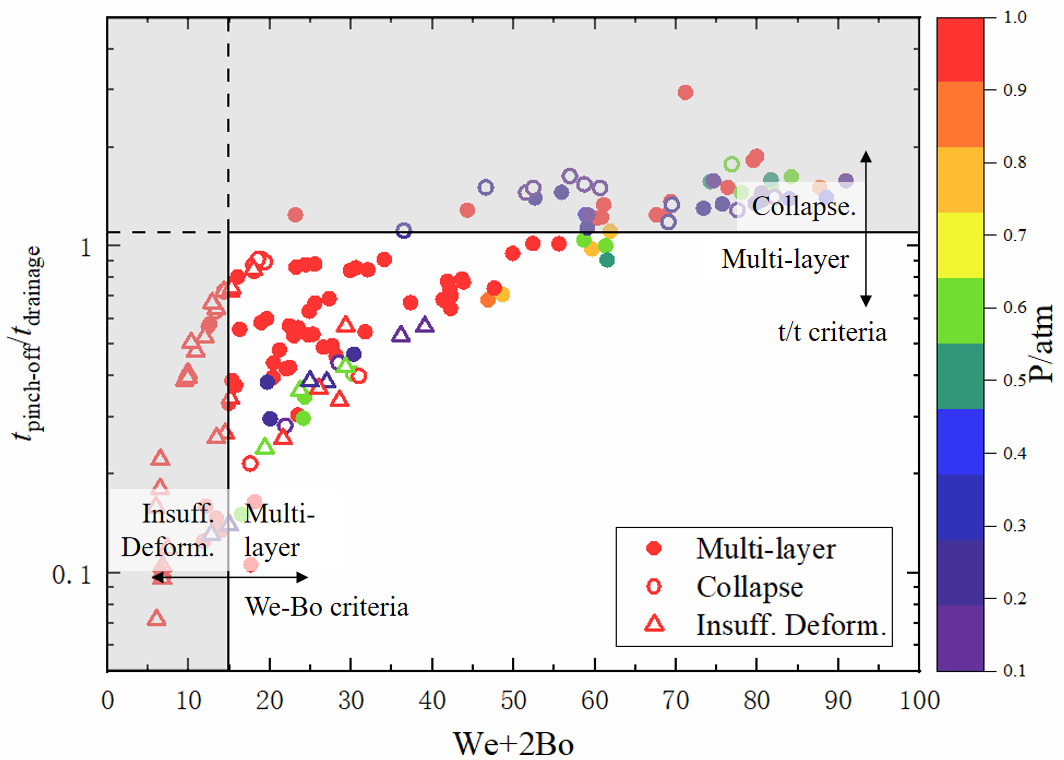
\includegraphics[width=0.48\linewidth]{figures/fig4_combined.png}
		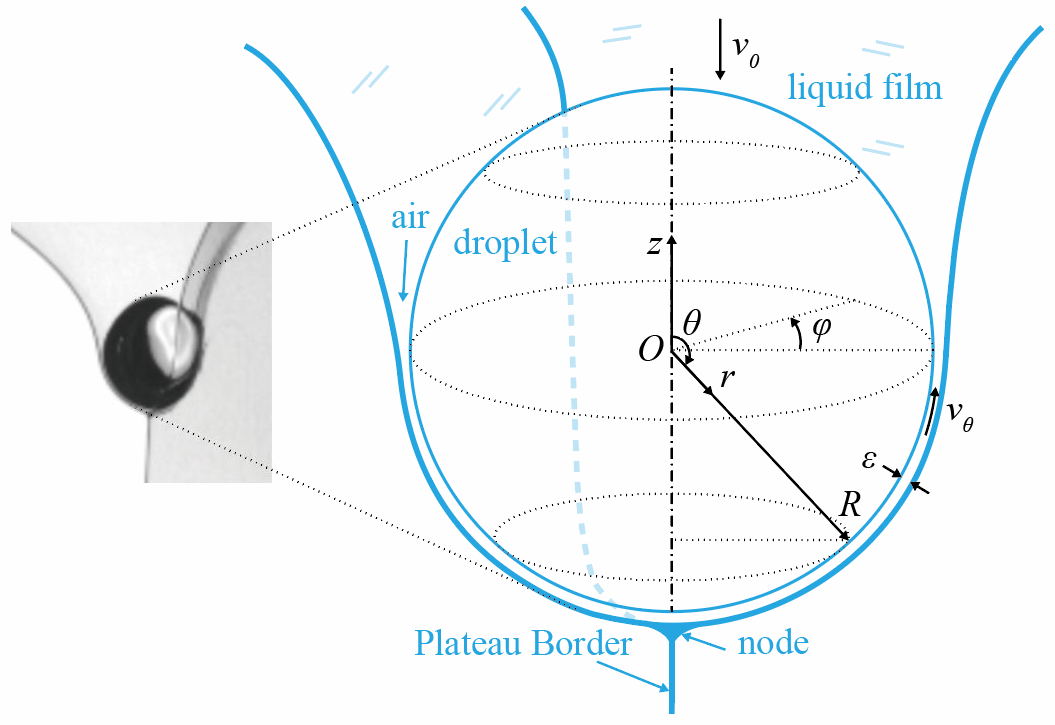
\includegraphics[width=0.48\linewidth]{figures/fig4_schematic.png}
		\caption{(a) Combined phase diagram in $(\text{We}+2\text{Bo}, t_p/t_d)$ space. The white region satisfies both the We--Bo energy criterion and the $t_p/t_d$ drainage criterion, containing 97\% of all successful packing outcomes. (b) Schematic of the gas film between the droplet and the deforming soap film in polar coordinates. Lubrication theory applies because $\varepsilon \sim 10~\mu\text{m} \ll R \sim 1$~mm.}
		\label{fig:combined}
	\end{center}
\end{figure}

{\noindent\textit{Parallel transport: droplet vs.\ rigid-sphere comparison.}}
A central result of this work is the parallel transport of deformable droplets and rigid spheres through the same PB channel. Rigid spheres (PP, PMMA, PS, POM) follow near-ballistic trajectories with acceleration within 3\% of $g$ and radius stability below 2\%, confirming that the PB channel itself does not introduce systematic measurement artifacts. The comparison reveals a fundamental dichotomy:\par

(1)~\textbf{PB entry.} Rigid spheres always enter the PB (no energy threshold), while droplets require $\text{We} + 2\text{Bo} > C_1$. The We--Bo criterion is thus a droplet-specific condition arising from the energy cost of deforming the soap films and entraining air.\par

(2)~\textbf{Gas-film dynamics.} Droplets entrain an air pocket during entry, forming a 1G1L structure with total gas volume $V_{\text{gas}} = V_p + V_f$ (pocket $+$ thin film). Rigid spheres have no gas pocket; any gas film is purely geometric, determined by the PB channel shape.\par

(3)~\textbf{Oscillation and collapse.} Droplets exhibit persistent shape oscillations during transport; rigid spheres show only geometric trajectory oscillations. Inner coalescence is exclusive to droplets, confirming that gas-film collapse is driven by droplet deformability.\par

{\noindent\textit{Coupled droplet--PB-film oscillation and cyclic gas shuttling.}}
During Stage~3 transport, the droplet undergoes persistent shape oscillations. Fourier analysis of the tracked radius $R(t)$ for two representative cases yields dominant frequencies $f = 60.6 \pm 0.4$~Hz (freefall, $R = 2.035$~mm) and $f = 68.6 \pm 0.7$~Hz (multi, $R = 1.936$~mm), with relative oscillation amplitudes $\delta R / R \approx 3.3$--$3.9\%$ and $R^2 > 0.99999$.\par

These frequencies lie near the range of Lamb's $n=3$ capillary mode for a free droplet, $\omega_n^2 = n(n-1)(n+2)\sigma/(\rho R^3)$, suggesting the PB film exerts weak constraint on the oscillating droplet. However, a complete physical picture requires accounting for the coupled dynamics of the droplet surface, the PB soap film, and the intervening gas film.\par

We develop a coupled oscillator model (full derivation in Supplementary Material). Three timescale comparisons are decisive. (i)~The gas pressure equilibration time $\tau_{\text{eq}} \sim 12\mu_a L^2/(P_{\text{amb}}\varepsilon_0^2) \sim 0.1$~ms is two orders of magnitude shorter than the oscillation period $T_{\text{osc}} \sim 15$~ms, ensuring spatially uniform $P_{\text{gas}}$ at every instant. (ii)~The PB film inertia is negligible: $\rho_f\delta_f/(\rho R) \sim 5\times10^{-4} \ll 1$, so the film responds quasi-statically to gas pressure. (iii)~The gas film is extremely stiff: $k_{\text{gas}}/k_{\text{cap}} \sim 4\pi P_{\text{amb}}R_0^2/(\sigma\varepsilon_0) \sim 10^6$, mechanically locking the PB film to the droplet surface.\par

Crucially, the $n=2$ ellipsoidal mode has a volume-preserving property: $\iint Y_{2m}(\theta,\phi)\,\sin\theta\,d\theta\,d\phi = 0$. Consequently, $n=2$ oscillations do \textit{not} change the total thin-film gas volume to first order---gas merely redistributes between the equator and the poles. The gas pocket at the droplet's top (a remnant of the pinch-off process) acts as a compliance reservoir, enabling gas to shuttle back and forth between the pocket and the thin-film region each cycle. This is a \textbf{reversible cyclic charge--discharge} process, not an RC decay: the pocket provides the extra gas capacity that sustains the film through many oscillation cycles.\par

The local film thickness oscillates as $\varepsilon(\theta,t) \approx \varepsilon_0[1 + \alpha P_2(\cos\theta)\sin(2\pi f t)]$, with $\alpha \sim 0.03$--$0.04$. At the equator during the oblate phase, $\varepsilon_{\min} \approx 0.98\,\varepsilon_0$. For $\varepsilon_0 \sim 10~\mu\text{m}$, this gives $\varepsilon_{\min} \sim 9.8~\mu\text{m}$, far above the van der Waals rupture threshold $\varepsilon_{\text{crit}} \sim 100$~nm, explaining why well-formed 1G1L structures survive for many oscillation cycles.\par

{\noindent\textit{Collapse mechanism.}}
Although the $n=2$ shuttling is largely reversible, net gas leakage accumulates over many cycles through three irreversible channels: (i)~\textbf{$h^3$ geometric rectification}---the lubrication flow nonlinearity gives a net outward bias $Q_{\text{out}}/Q_{\text{in}} \sim (1+6\alpha) \sim 1.2$ per cycle; (ii)~\textbf{bottom-edge leakage} at the droplet--PB--liquid triple line during compression phases; and (iii)~\textbf{pocket symmetry breaking}---the pocket at $\theta \approx 0$ creates preferential gas exchange paths, leaving the equatorial and bottom film regions less replenished.\par

Gravitational drainage is negligible under these conditions: the gravitational drainage time $\tau_g \sim \mu R/(\rho g \varepsilon_0^2) \sim 2.4$~s far exceeds the PB transit time $t_{\text{trans}} = L_{\text{PB}}/v \sim 0.1$~s ($\tau_g/t_{\text{trans}} \sim 24$), and the oscillation-driven gas velocity exceeds the gravitational drainage velocity by a factor $v_{\text{osc}}/v_g \sim 5.4$.\par

We characterize the collapse propensity by a dimensionless collapse number:
\begin{equation}
\mathcal{C} \equiv \alpha^3 \times \frac{f\,t_{\text{trans}}}{V_p/V_f},
\label{eq:collapse}
\end{equation}
where $\alpha = \delta R/R$ is the relative oscillation amplitude, $f\,t_{\text{trans}}$ is the number of oscillation cycles during transit, and $V_p/V_f$ is the pocket-to-film volume ratio. Collapse occurs when $\mathcal{C} > \mathcal{C}_{\text{crit}}$, where $\mathcal{C}_{\text{crit}}$ is a geometry-dependent constant to be calibrated from direct $\varepsilon$ measurements.\par

For rigid spheres, $\alpha = 0 \Rightarrow \mathcal{C} = 0$, consistent with the complete absence of inner-coalescence events across all rigid-sphere experiments. This provides independent confirmation that droplet deformability is the root cause of the collapse mechanism.\par

% ======================================================================
\textcolor{cyan}{\textbf{Conclusions}}\par

We have demonstrated that a single, well-defined Plateau border in a 3D-printed frame enables controllable antibubble generation with 97\% predictable outcomes across 199 experiments.\par

By comparing droplet and rigid-sphere transport through the same PB channel, we have isolated the geometric contribution of the PB (universal low-resistance transport) from droplet-specific gas-film dynamics (air entrainment, shape oscillation, and inner coalescence).\par

Two dimensionless criteria govern antibubble formation: the We--Bo energy relation $[\text{We} + 2\text{Bo} = 0.038 \pm 0.004]$ determines whether a droplet can enter the PB, and the characteristic-time ratio $t_p/t_d < 1$ determines whether the gas film survives pinch-off. The PB geometry provides a twofold efficiency advantage over horizontal-interface methods ($C_1/C_1' \approx 0.53$).\par

Droplet shape oscillations during transport follow Lamb capillary modes. A coupled droplet--PB-film model reveals that the $n=2$ mode preserves gas-film volume to first order, enabling reversible cyclic gas shuttling sustained by the post-pinch-off gas pocket. A collapse number $\mathcal{C} \equiv \alpha^3 f t_{\text{trans}}/(V_p/V_f)$ captures the net effect of irreversible leakage mechanisms. Rigid-sphere control experiments confirm that inner coalescence is exclusive to deformable droplets.\par

This work provides a predictive framework for antibubble generation and establishes the single-PB platform as a controlled experimental system for studying confined transport phenomena in foam microchannels, with implications for drug delivery, microfluidic transport, and microgravity fluid management.\par

\begin{acknowledgments}
We gratefully acknowledge insightful discussions with H.~A.~Stone, C.~Sun, and L.~Bai. We acknowledge support on fluid data provided by Y.~Y.~Duan. We acknowledge financial support by the National Natural Science Foundation of China (NSFC, No.~52076120 and No.~52079066), the State Key Laboratory of Hydroscience and Engineering, and the Creative Seed Fund of Shanxi Research Institute for Clean Energy, Tsinghua University.
\end{acknowledgments}

\bibliography{references}

\end{document}
